\documentclass[totpages,helvetica,openbib,spanish]{europecv}
\usepackage[T1]{fontenc}
\usepackage{graphicx}
\usepackage[a4paper,top=1.27cm,left=1cm,right=1cm,bottom=2cm]{geometry}
\usepackage[spanish]{babel}
\usepackage{bibentry}
\usepackage{url}
\usepackage{enumitem}
\setlist{nolistsep}

\renewcommand{\normalsize}{\fontsize{2.9mm}{3.1mm}\selectfont}

\ecvname{Diego Russo}
\ecvaddress{Calle G. Garibaldi 40, 05021, Acquasparta (TR), Italia}
\ecvtelephone[+39 334 5873886]{+39 0744 930614}
\ecvemail{\url{diegor.it@gmail.com} - Personal, Gtalk, MSN \\& \url{diego.russo@forinicom.it} - Forinicom S.r.l.}
\ecvhomepage{\url{http://www.diegor.it}}
\ecvnationality{Italiano}
\ecvdateofbirth{30 de Abril de 1983}
\ecvgender{Varo}
\ecvbeforepicture{\raggedleft}
\ecvpicture[width=3cm]{../images/diegor.jpg}
\ecvafterpicture{\ecvspace{-3cm}} 
\ecvfootnote{Para mas informaci\'on: \url{http://europass.cedefop.eu.int}\\
\textcopyright~European Communities, 2003.}

\begin{document}
    \begin{center}
        \hspace{1pt}
        \vspace{2cm}
    
        {\scshape \textbf{\Huge Diego Russo}}
    
        \vspace{1cm}
    
        {\scshape \textbf{\large \underline{Curriculum Vitae}}}
    
        \vspace{0.25cm}
    
        actualizaci\'on \emph{\textbf{20 de Marzo 2010}}
        
        \vspace{2cm}
        
        \begin{figure}[htbp] 
            \begin{center} 
                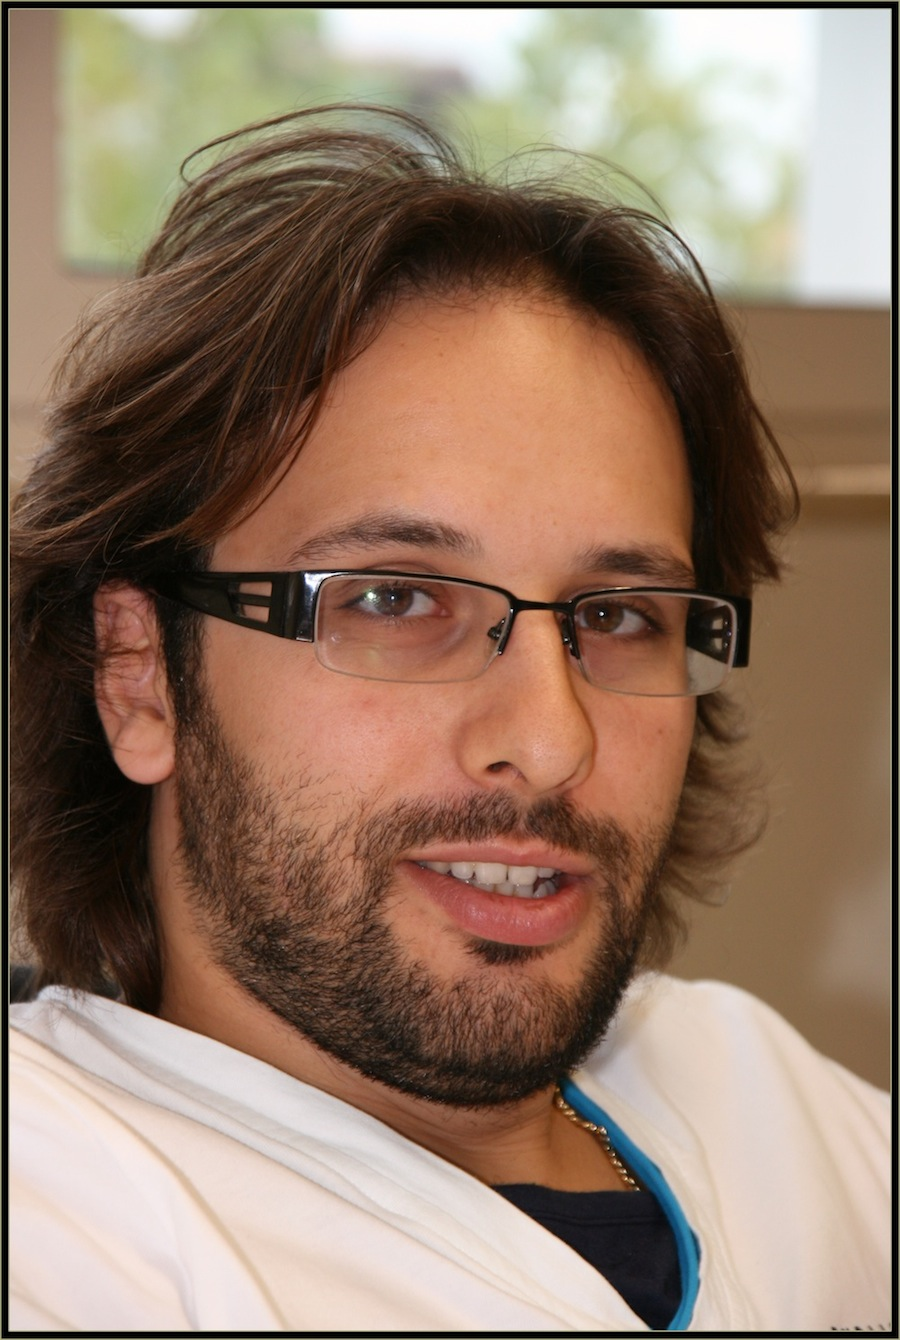
\includegraphics[width=10cm]{../images/io.jpg}
            \end{center} 
        \end{figure}
        
    \end{center}
\pagebreak
\selectlanguage{spanish}

\begin{europecv}
\ecvpersonalinfo[5pt]

\ecvitem{\large\textbf{Empleo deseado / campo profesional}}{\large\textbf{Programador Python, Django. Ingeniero de sistemas Linux, OSX. Tambi\'en abierto a otras propuestas con la posibilidad de crecimiento profesional y personal.}}

\ecvsection{Experiencia laboral}

\ecvitem{Fechas}{\textbf{De 26 Abril 2008 a la actualidad   }}
\ecvitem{Puesto o cargo ocupados}{Programador, ingeniero de sistema (aprendizaje de los trabajadores con un contrato a tiempo parcial, 25 horas)}
\ecvitem{Tareas y responsabilidades principales}{Desarrollo de un proyecto que tiene como objetivo ofrecer conectividad y servicios integrados (v\'ideo, VoIP) a las administraciones p\'ublicas, empresas y particulares. Puntos en el marco del contrato:
\begin{itemize}
    \item conocer los productos y los servicios y el entorno empresarial: redes a mallas y redes jer\'arquicas, los servicios de VoIP y video vigilancia, seguridad de redes cableadas e inal\'ambricas;
    \item conocer y aplicar las bases cient\'ificas y t\'ecnicas de profesionalismo;
    \item conocer y utilizar t\'ecnicas y m\'etodos de trabajo, con especial referencia al desarrollo de software y documentaci\'on de c\'odigo;
    \item conocer y utilizar herramientas y tecnolog\'ias de trabajo (equipos, maquinaria y herramientas), sobre todo entorno de desarrollo Linux, desarrollo de la plataforma Linux/OSX, lenguajes de programaci\'on Python y PostgreSQL/MySQL;
    \item conocer y utilizar las medidas de seguridad individual y la protecci\'on del medio ambiente;
    \item conocer las innovaciones de producto, proceso, contexto y sector.
\end{itemize}
Tambi\'en desarroll\'e aplicaciones en python y python-django tanto para el trabajo diario del departamento t\'ecnico y no es la investigaci\'on pura y el desarrollo. En este contexto he vuelto a implementado un servidor para gestionar el \textbf{servicio de hotspot}}
\ecvitem{Nombre y direcci\'on del empleador}{Forinicom srl, Calle del Popolo, 9 Bastia Umbra, 06083, 0758001868, \url{http://www.forinicom.it}}
\ecvitem[10pt]{Tipo de empresa o sector}{Telecomunicaciones}

\ecvitem{Fechas}{\textbf{De 03 Septiembre 2009 a la actualidad}}
\ecvitem{Puesto o cargo ocupados}{Programador (contrato del proyecto, a tiempo parcial)}
\ecvitem{Tareas y responsabilidades principales}{Desarrollo de una aplicaci\'on de gesti\'on para el municipio de Bettona en Django, Python, PostgreSQL, Linux, Apache, para la informatizaci\'on de los servicios para la gesti\'on de datos maestros, as\'i como la construcci\'on y las pr\'acticas de planificaci\'on y el c\'alculo del impuesto sobre actualizaciones ICI datos catastrales. Utilizo de  un servidor de control de versiones (GIT). Tambi\'en en esta etapa fue la realizaci\'on del producto a su comercializaci\'on.}
\ecvitem{Nombre y direcci\'on del empleador}{Consorzio Miles - Servizi Integrati, CF 04881101002, Calle Rocca di Papa 21, Roma}
\ecvitem[10pt]{Tipo de empresa o sector}{Servicios integrados para la administraci\'on p\'ublica}

\ecvitem{Fechas}{\textbf{De 11 Diciembre 2006 a 31 Agosto 2008}}
\ecvitem{Puesto o cargo ocupados}{Programmatore (lavoratore con contratto a progetto, full-time)}
\ecvitem{Tareas y responsabilidades principales}{Desarrollo de una aplicaci\'on de gesti\'on para el municipio de Bettona en Django, Python, PostgreSQL, Linux, Apache, para la informatizaci\'on de los servicios para la gesti\'on de datos maestros, as\'i como la construcci\'on y las pr\'acticas de planificaci\'on y el c\'alculo del impuesto sobre actualizaciones ICI datos catastrales. Utilizo de  un servidor de control de versiones (SVN), con su interfaz web (Trac) para gestionar los tickets.}
\ecvitem{Nombre y direcci\'on del empleador}{Consorzio Miles - Servizi Integrati, CF 04881101002, Calle Rocca di Papa 21, Roma}
\ecvitem[10pt]{Tipo de empresa o sector}{Servicios integrados para la administraci\'on p\'ublica}

\ecvitem{Fechas}{\textbf{De 30 Julio 2006 a 30 Diciembre 2006}}
\ecvitem{Puesto o cargo ocupados}{Estudiante de licenciatura (Wireless Broadband Network)}
\ecvitem{Tareas y responsabilidades principales}{Wireless Broadband Network - proyecto \textbf{WeConnect} - Banda ancha sobre redes inal\'ambricas:
    \begin{itemize}
        \item amplio conocimiento de la red inal\'ambrica y su funcionamiento;
        \item buen conocimiento de las leyes sobre el Wi-Fi
        \item excelente conocimiento del sistema de Router (www.mikrotik.com)
        \item el conocimiento de protocolo y FreeRADIUS Servidor AAA
        \item la administraci\'on de los servicios de red diferentes: mail (postfix), servidor web (Apache), DNS (pdns), firewall (iptables), bases de datos (PostgreSQL), puntos de acceso (chillispot), sistema operativo Debian, Voyage (OSX para sistemas embebidos basados en Debian)
    \end{itemize}}
\ecvitem{Nombre y direcci\'on del empleador}{WEDOIT s.a.s. - Calle Protomartiri Francescani,26 - 06088 Assisi (PG)}
\ecvitem[10pt]{Tipo de empresa o sector}{Servicios integrados para la administraci\'on p\'ublica}

\ecvitem{Fechas}{\textbf{De 14 Noviembre 2005 a 30 Mayo 2006}}
\ecvitem{Puesto o cargo ocupados}{Formaci\'on (S.E.O. Search Engine Optimization)}
\ecvitem{Tareas y responsabilidades principales}{\vspace{-2mm}
    \begin{itemize}
        \item Conocimientos de SEO y su mecanismos. Optimizar un sitio para S.E.O.
        \item Pageranking t\'ecnicas y popularidad de enlaces
        \item Sistemas de un servidor virtual basado en Debian
        \item Estudio del lenguaje de programaci\'on Python, con la aplicaci\'on de algunos SEO orientado a la aplicaci\'on
        \item Estudio del lenguaje de programaci\'on PHP, para desarrollar algunas aplicaciones orientadas a SEO
    \end{itemize}}
\ecvitem{Nombre y direcci\'on del empleador}{WEDOIT s.a.s. - Calle Protomartiri Francescani,26 - 06088 Assisi (PG)}
\ecvitem[10pt]{Tipo de empresa o sector}{Soluciones informaticas}

\ecvitem{Fechas}{\textbf{Marzo 2002}}
\ecvitem{Puesto o cargo ocupados}{Formaci\'on (formaci\'o del proyecto IFS, Impresa Formativa Simulata)}
\ecvitem{Tareas y responsabilidades principales}{Gesti\'on de la red dentro de la empresa.}
\ecvitem{Nombre y direcci\'on del empleador}{IOSA CARLO S.r.l. - 05100 TERNI - Calle Pallotta n. 7 - Tel. +3907442460 - Fax +390744246035 - P.IVA 00072550551 - \url{http://www.iosacarlo.com} - \url{iosacarlo@iosacarlo.com}}
\ecvitem[10pt]{Tipo de empresa o sector}{Empresa de tratamiento de residuos}

\ecvsection{Educaci\'on / formaci\'on recibida}

\ecvitem{Fechas}{\textbf{De Ottobre 2008 a la actualidad}}
\ecvitem{T\'itulo obtenido}{Iscritto alla specializzazione di Informatica, indirizzo di ``Sicurezza Informatica''}
\ecvitem{Principales materias o capacidades profesionales aprendidas}{Sostenuti i seguenti esami con relativa votazione:\begin{itemize}
    \item Simulazione: 30 e lode
    \item Programmazione Avanzata: 30 e lode
    \item Sistemi operativi avanzati: 30 e lode
    \item Laboratorio di Sistemi operativi avanzati: 30 e lode
\end{itemize}}
\ecvitem{Nombre y tipo de centro que ha impartido la ense\~nanza}{Universit\'a degli studi di Perugia, Dipartimento di Informatica}
\ecvitem[10pt]{Nivel alcanzado en una clasificaci\'on nacional o internacional}{-}

\ecvitem{Fechas}{\textbf{De 17 Febrero 2010 a la actualidad}}
\ecvitem{T\'itulo obtenido}{Iscritto al 4$^\circ$ modulo di lingua spagnola}
\ecvitem{Principales materias o capacidades profesionales aprendidas}{I livelli raggiunti in questo modulo sono i seguenti:
\begin{itemize}
    \item capire gli elementi principali in un discorso chiaro in lingua standard su argomenti familiari
    \item riuscire a descrivere esperienze ed avvenimenti, motivare e spiegare progetti
    \item affrontare molte delle situazioni che si possono presentare viaggiando in una zona dove si parla la lingua
\end{itemize}}
\ecvitem{Nombre y tipo de centro que ha impartido la ense\~nanza}{Istituto comprensivo ``Volumnio'' Ponte San Giovanni - Perugia}
\ecvitem[10pt]{Nivel alcanzado en una clasificaci\'on nacional o internacional}{-}

\ecvitem{Fechas}{\textbf{De Agosto 2009 a Marzo 2010}}
\ecvitem{T\'itulo obtenido}{Pubblicazione del paper \textbf{``The AES implentation based on OpenCL for multi/many core architecture''}}
\ecvitem{Principales materias o capacidades profesionales aprendidas}{Preparazione e pubblicazione del paper ``The AES implentation based on OpenCL for multi/many core architecture'' per l'annuale conferenza ICCSA 2010 (\url{www.iccsa.org}) alla Sangyo University, Fukuoka in Giappone. Il paper tratta di un' implementazione di AES eseguito su core GPU NVIDIA/ATI.}
\ecvitem{Nombre y tipo de centro que ha impartido la ense\~nanza}{Universit\'a degli studi di Perugia, Dipartimento di Informatica}
\ecvitem[10pt]{Nivel alcanzado en una clasificaci\'on nacional o internacional}{-}

\ecvitem{Fechas}{\textbf{De 14 Octubre 2009 al 12 Febrero 2010}}
\ecvitem{T\'itulo obtenido}{Attestato di frequenza di 42 ore su 50 del 3$^\circ$ modulo di lingua spagnola}
\ecvitem{Principales materias o capacidades profesionales aprendidas}{I livelli raggiunti in questo modulo sono i seguenti:
\begin{itemize}
    \item comprendere frasi ed espressioni di uso frequente relativi ad ambiti di immediata rilevanza
    \item saper descrivere in termini semplici aspetti della propria storia e delle proprie esperienze
    \item saper parlare dell'ambiente circostante e saper esprimere bisogni, intenzioni e previsioni
\end{itemize}}
\ecvitem{Nombre y tipo de centro que ha impartido la ense\~nanza}{Istituto comprensivo ``Volumnio'' Ponte San Giovanni - Perugia}
\ecvitem[10pt]{Nivel alcanzado en una clasificaci\'on nacional o internacional}{-}

\ecvitem{Fechas}{\textbf{De Agosto 2007 a Agosto 2008}}
\ecvitem{T\'itulo obtenido}{Pubblicazione del libro \textbf{UbuntuSemplice 7.10} con conseguente donazione a Canonical Ltd.}
\ecvitem{Principales materias o capacidades profesionales aprendidas}{\vspace{-2mm}
\begin{itemize}
    \item Contributor, autore di molti capitoli e sistemista del sistema informatico per \url{http://www.ubuntusemplice.org/}
    \item Amministrazione di un server virtuale Debian
    \item Configurazione ed utilizzo del software collaborativo MediaWiki per la stesura e composizione del libro.
    \item Configurazione del server web apache
    \item Configurazione di una mailing list per la gestione dei capitoli del libro con gli altri contributor
\end{itemize}}
\ecvitem{Nombre y tipo de centro que ha impartido la ense\~nanza}{Progetto Ubuntusemplice - \url{http://www.ubuntusemplice.org/)}}
\ecvitem[10pt]{Nivel alcanzado en una clasificaci\'on nacional o internacional}{Ottima conoscenza del sistema operativo Ubuntu}

\ecvitem{Fechas}{\textbf{De Febrero 2007 a Julio 2007}}
\ecvitem{T\'itulo obtenido}{Patente di operatore di stazione di radioamatore di classe A}
\ecvitem{Principales materias o capacidades profesionales aprendidas}{Corso per aspiranti radioamatori:
\begin{itemize}
    \item Ottima conoscenza delle basi della radiotecnica
    \item Ottima conoscenza delle apparecchiature radio e del loro funzionamento
    \item Conoscenza delle basi della fisica e chimica (magnetismo,  elettromagnetismo)
\end{itemize}}
\ecvitem{Nombre y tipo de centro que ha impartido la ense\~nanza}{C.I.S.A.R. Sezione di Foligno}
\ecvitem[10pt]{Nivel alcanzado en una clasificaci\'on nacional o internacional}{IDONEO, Nominativo internazionale \textbf{IZ0OVB}}

\ecvitem{Fechas}{\textbf{De 19 Marzo 2007 a 23 Marzo 2007}}
\ecvitem{T\'itulo obtenido}{Attestato di partecipazione al corso di lingua spagnola}
\ecvitem{Principales materias o capacidades profesionales aprendidas}{\vspace{-2mm}
\begin{itemize}
    \item Grammatica di base della lingua spagnola
    \item Cultura generale spagnola
\end{itemize}}
\ecvitem{Nombre y tipo de centro que ha impartido la ense\~nanza}{Inhispania Intlance S.L / CIF:B83744847 , Montera 10-12, 1-1. 28013, Madrid (Spain)}
\ecvitem[10pt]{Nivel alcanzado en una clasificaci\'on nacional o internacional}{Valutazioni\footnote{Valutazione in accordo con il ``Common European Framework of Reference for Languages''}:
\begin{itemize}
    \item Espressione orale: A2
    \item Espressione scritta: A2
    \item Comprensione orale: A2
    \item Comprensione scritta: A2
    \item Interazione orale: A2
\end{itemize}}

\ecvitem{Fechas}{\textbf{03-10-25 Marzo 2007}}
\ecvitem{T\'itulo obtenido}{Attestato di partecipazione al corso su tecnologie Microsoft}
\ecvitem{Principales materias o capacidades profesionales aprendidas}{Gli argomenti trattati al corso sono stati:
\begin{itemize}
    \item .NET Framework Architeture (2.0)
    \item ADO.NET
    \item ASP.NET (web forms, Page, controlli, sicurezza)
    \item C\#
    \item Web Service
    \item Ajax.net
    \item Microsoft Visual Studio 2005
\end{itemize}}
\ecvitem{Nombre y tipo de centro que ha impartido la ense\~nanza}{O.S.MO.S.IT, Via Strozzacapponi, 85, 06071 Castel del Piano (Pg)}
\ecvitem[10pt]{Nivel alcanzado en una clasificaci\'on nacional o internacional}{Conoscenza di base della programmazione Microsoft}

\ecvitem{Fechas}{\textbf{De Septiembre 2006 a Febrero 2007}}
\ecvitem{T\'itulo obtenido}{Pubblicazione del libro \textbf{UbuntuSemplice 6.06} con conseguente donazione a Canonical Ltd.}
\ecvitem{Principales materias o capacidades profesionales aprendidas}{\vspace{-2mm}
\begin{itemize}
    \item Contributor, autore di molti capitoli e sistemista del sistema informatico per \url{http://www.ubuntusemplice.org/}
    \item Amministrazione di un server virtuale Debian
    \item Configurazione ed utilizzo del software collaborativo MediaWiki per la stesura e composizione del libro.
    \item Configurazione del server web apache
    \item Configurazione di una mailing list per la gestione dei capitoli del libro con gli altri contributor
\end{itemize}}
\ecvitem{Nombre y tipo de centro que ha impartido la ense\~nanza}{Progetto Ubuntusemplice - \url{http://www.ubuntusemplice.org/)}}
\ecvitem[10pt]{Nivel alcanzado en una clasificaci\'on nacional o internacional}{Ottima conoscenza del sistema operativo Ubuntu}

\ecvitem{Fechas}{\textbf{01-02-03 Diciembre 2006}}
\ecvitem{T\'itulo obtenido}{Attestato di partecipazione al corso sulle certificazioni ISO}
\ecvitem{Principales materias o capacidades profesionales aprendidas}{Corso di formazione sulla sicurezza e certificazioni ISO:
\begin{itemize}
    \item ISO 27001:2005
    \item Politica per la sicurezza delle informazioni
    \item Analisi dei rischi (RA)
    \item Analisi dei controlli della ISO 17799:2005
    \item Trattamento dei rischi (RTP)
    \item Processo di certificazione
    \item Panorama delle certificazioni  per gli audit
    \item Piano di audit e checklist
    \item Rapporto di audit
    \item Uno sguardo alle future certificazioni
\end{itemize}}
\ecvitem{Nombre y tipo de centro que ha impartido la ense\~nanza}{WEDOIT s.a.s. - Via Protomartiri Francescani, 26 - 06088 Assisi (PG)}
\ecvitem[10pt]{Nivel alcanzado en una clasificaci\'on nacional o internacional}{Conoscenza dei processi di certificazione ISO}

\ecvitem{Fechas}{\textbf{De Octubre 2002 a Noviembre 2006}}
\ecvitem{T\'itulo obtenido}{\textbf{Laurea triennale (nuovo ordinamento) in Informatica}}
\ecvitem{Principales materias o capacidades profesionales aprendidas}{Laurea triennale in informatica, \textbf{indirizzo ``Reti di computer''}:
\begin{itemize}
    \item Matematica (analitica e discreta)
    \item Programmazione (C, Java, Php, html, xml, xsl, dtd, Pascal, scripting bash e csh, VB.NET, VRML)
    \item DataBase (Mysql, MS Access e loro interazioni con linguaggi di programmazione)
    \item Reti (ATM, xDSL, Mpls, X.25, Frame Relay), tipologie (wireless, wired) e loro interazione
    \item Conoscenza di sistemi multimediali
    \item Cenni di calcolo parallelo (mpi)
\end{itemize}}
\ecvitem{Nombre y tipo de centro que ha impartido la ense\~nanza}{Universit\'a degli studi di Perugia, Dipartimento di Informatica}
\ecvitem[10pt]{Nivel alcanzado en una clasificaci\'on nacional o internacional}{\textbf{102/110}}

\ecvitem{Fechas}{\textbf{De Septiembre 1996 a Junio 2002}}
\ecvitem{T\'itulo obtenido}{\textbf{Diploma in ragioniere programmatore (progetto Mercurio)}}
\ecvitem{Principales materias o capacidades profesionales aprendidas}{Materie previste dal percorso di studio dell'Istituto Tecnico Commerciale, definito dal Ministero dell'Istruzione, ovvero:
\begin{itemize}
    \item Scienze della Materia
    \item Matematica e Laboratorio
    \item Scienze della Natura
    \item Trattamento Testi e Dati
    \item Seconda lingua straniera (Francese)
    \item Diritto ed Economia
    \item Economia Aziendale
    \item Economia Politica e Scienza delle Finanze
    \item Lingua e letteratura italiana
    \item Storia
    \item Informatica Gestionale
    \item Matematica applicata
    \item Prima lingua straniera (Inglese)
    \item Diritto
\end{itemize}}
\ecvitem{Nombre y tipo de centro que ha impartido la ense\~nanza}{Ministero della Pubblica Istruzione - I.T.C. ``Federico Cesi'', Terni}
\ecvitem[10pt]{Nivel alcanzado en una clasificaci\'on nacional o internacional}{\textbf{85/100}}

\ecvitem{Fechas}{\textbf{De 2001 a 2002}}
\ecvitem{T\'itulo obtenido}{Attestato di frequenza al Progetto Nazionale IFS (\textbf{Impresa Formativa Simulata})}
\ecvitem{Principales materias o capacidades profesionales aprendidas}{Simulazione di un'impresa di smaltimento rifiuti, affiancati dall'impresa Iosa Carlo S.r.l. (\url{http://www.iosacarlo.com}).
Nell'ambito del progetto ho coordinato il lavoro di tutti gli studenti, realizzando l'organigramma dell'azienda simulata e programmando il sito dell'azienda.}
\ecvitem{Nombre y tipo de centro que ha impartido la ense\~nanza}{Ministero della Pubblica Istruzione - I.T.C. ``Federico Cesi'', Terni}
\ecvitem[10pt]{Nivel alcanzado en una clasificaci\'on nacional o internacional}{-}

\ecvitem{Fechas}{\textbf{De 24 Septiembre 2001 a 14 Octubre 2001}}
\ecvitem{T\'itulo obtenido}{Attestato di frequenza al corso come tutor}
\ecvitem{Principales materias o capacidades profesionales aprendidas}{Svoltasi l'attivit\'a di tutor/referente di un gruppo di altri 6 studenti/tutor, per le attivit\'a di POTENZIAMENTO DI ITALIANO delle prime classi, in ambito del progetto ``Accoglienza, Recupero, Potenziamento nelle Prime Classi''.
L'attivit\'a \'e consistita nell'affiancare i Docenti di Lettere al fine di offrire un valido supporto agli alunni delle Prime Classi nell'utilizzo del Computer, per poter eseguire attivit\'a di approfondimento con il mezzo multimediale, attraverso esercitazioni con un CD-Rom di Grammatica.}
\ecvitem{Nombre y tipo de centro que ha impartido la ense\~nanza}{Ministero della Pubblica Istruzione - I.T.C. ``Federico Cesi'', Terni}
\ecvitem[10pt]{Nivel alcanzado en una clasificaci\'on nacional o internacional}{Acquisite ottime capacit\'a relazionali, organizzative ed ottime competenze nell'insegnamento di materie tecniche}

\ecvitem{Fechas}{\textbf{De 7 Diciembre 2001 a 09 Diciembre 2001}}
\ecvitem{T\'itulo obtenido}{Attestato di frequenza del ``Pluto Meeting 2001''}
\ecvitem{Principales materias o capacidades profesionales aprendidas}{Partecipazione all'organizzazione del ``Pluto Meeting 2001'', tenuto presso il suddetto istituto.}
\ecvitem{Nombre y tipo de centro que ha impartido la ense\~nanza}{Ministero della Pubblica Istruzione - I.T.C. ``Federico Cesi'', Terni}
\ecvitem[10pt]{Nivel alcanzado en una clasificaci\'on nacional o internacional}{-}

\ecvitem{Fechas}{\textbf{De 26 Marzo 2001 a 02 Abril 2001}}
\ecvitem{T\'itulo obtenido}{Attestato di frequenza alla ``XI Settimana della cultura scientifica e tecnologica''}
\ecvitem{Principales materias o capacidades profesionales aprendidas}{Partecipazione alla ``XI Settimana della cultura scientifica e tecnologica'', realizzando sia la locandina che il programma provinciale della settimana delle scienze in Adobe Photoshop 5.5 ed in Corel Draw 8.0, impegnandosi sia in orario curriculare che extra-curriculare pomeridiano con grande devozione, senso della responsabilit\'a, fungendo anche da punto di riferimento per tutti gli studenti del biennio che hanno partecipato al progetto.}
\ecvitem{Nombre y tipo de centro que ha impartido la ense\~nanza}{Ministero della Pubblica Istruzione - I.T.C. ``Federico Cesi'', Terni}
\ecvitem[10pt]{Nivel alcanzado en una clasificaci\'on nacional o internacional}{-}

\ecvitem{Fechas}{\textbf{A\~no 2001}}
\ecvitem{T\'itulo obtenido}{Attestato di frequenza come tutor al corso di alfabetizzazione di computer per over 65}
\ecvitem{Principales materias o capacidades profesionales aprendidas}{Corso di alfabetizzazione di computer di base in funzione di tutor di 40 ore complessive ad un gruppo di 30 persone, con et\'a superiore al 65 anni.
Ho svolto inoltre il ruolo di coordinatore del progetto stilando il programma e coordinando i miei colleghi.}
\ecvitem{Nombre y tipo de centro que ha impartido la ense\~nanza}{Ministero della Pubblica Istruzione - I.T.C. ``Federico Cesi'', Terni}
\ecvitem[10pt]{Nivel alcanzado en una clasificaci\'on nacional o internacional}{-}

\ecvitem{Fechas}{\textbf{A\~no 2001}}
\ecvitem{T\'itulo obtenido}{Attestato di frequenza al corso di informatica}
\ecvitem{Principales materias o capacidades profesionales aprendidas}{Corso di informatica di base in funzione di tutor (progetto 20 Studenti) di 30 ore complessive su applicazioni office (Word, Excel) ed Internet}
\ecvitem{Nombre y tipo de centro que ha impartido la ense\~nanza}{Ministero della Pubblica Istruzione - I.T.C. ``Federico Cesi'', Terni}
\ecvitem[10pt]{Nivel alcanzado en una clasificaci\'on nacional o internacional}{-}

\ecvitem{Fechas}{\textbf{16-17-18 Noviembre 2000}}
\ecvitem{T\'itulo obtenido}{Attestato di frequenza all'Exposcuola 2000}
\ecvitem{Principales materias o capacidades profesionales aprendidas}{Exposcuola - Salone del confronto tra le proposte formative dell'Europa e del Mediterraneo - Paestum hotel Ariston}
\ecvitem{Nombre y tipo de centro que ha impartido la ense\~nanza}{Ministero della Pubblica Istruzione - I.T.C. ``Federico Cesi'', Terni}
\ecvitem[10pt]{Nivel alcanzado en una clasificaci\'on nacional o internacional}{-}

\ecvitem{Fechas}{\textbf{De 1997 a 1998}}
\ecvitem{T\'itulo obtenido}{Attestato di frequenza}
\ecvitem{Principales materias o capacidades profesionales aprendidas}{Corso di base sulla multimedialit\'a (progetto 20 studenti) per un totale di 25 ore.}
\ecvitem{Nombre y tipo de centro que ha impartido la ense\~nanza}{{Ministero della Pubblica Istruzione - I.T.C. ``Federico Cesi'', Terni}}
\ecvitem[10pt]{Nivel alcanzado en una clasificaci\'on nacional o internacional}{-}

\ecvsection{Capacidades y competencias personales}

\ecvmothertongue[5pt]{Italiano}
\ecvitem{\large Otro(s) idioma(s)}{\textbf{Ingl\'es, Espa\~nol}}
\ecvlanguageheader{(*)}
\ecvlanguage{Ingl\'es}{\ecvBOne}{\ecvBOne}{\ecvATwo}{\ecvATwo}{\ecvBOne}
\ecvlastlanguage{Espa\~nol}{\ecvBOne}{\ecvBOne}{\ecvATwo}{\ecvATwo}{\ecvBOne}
\ecvlanguagefooter[10pt]{(*)}

\ecvitem[10pt]{Capacidades y competencias sociales}{Ottime capacit\'a di relazionarsi con colleghi e collaboratori. Socievole, simpatico e con buone doti comunicative. Propenso al lavoro in team. Il mio sito \'e fonte di contatti e scambi sociali continui con altre persone tecniche e meno techiche.)}
\ecvitem[10pt]{Capacidades y competencias organizativas}{Capacit\'a di lavorare in maniera efficiente in diverse situazioni.}
\ecvitem[10pt]{Capacidades y competencias inform\'aticas}{Dada mi pasi\'on por la inform\'atica en general con los a\'nos he desarrollado una serie de competencias que var\'ian en muchas \'areas de la misma.

Desde mi primer ordenador ten\'ia una pasi\'on por el mundo del c\'odigo abierto y todo lo que le concierne: de hecho me las arregl\'e las m\'aquinas con las distribuciones de \textbf{Linux} como RedHat 7.3, Slackware 7.1 hasta llegar a las m\'aquinas de Debian (desde la versi\'on 3.0 a las actuales ).
A trav\'es de esta experiencia que he adquirido cierta habilidad y conocimiento en la administraci\'on de Linux: comandos bash, configurar y compilar el kernel, los servicios de red, los patches para el n\'ucleo, el lenguaje C. Adem\'as de regular el uso de \textbf{Linux/OSX} para el uso diario. Teniendo en cuenta el uso continuado y mi pasi\'on por los ordenadores que tengo, estudio en profundidad de los sistemas UNIX basados en OSX.

\textbf{Tambi\'en tengo una pasi\'on por la programaci\'on:} conozco a muchos idiomas (de programaci\'on) en zonas muy diferentes entre s\'i como Python, C, PHP, Java, LSL (Linden Scripting Language). La LSL estudi\'e durante mis actividades en \textbf{Second Life}, de hecho he trabajado en varios proyectos italianos en el metaverso como \url{http://www.secundavita.it} As\'is, Mil\'an y Marostica en el proyecto Vera. Conocimiento de las aplicaciones gr\'aficas (Gimp, Photoshop) y herramientas de oficina como OpenOffice, org y iWork (para OSX)}
\ecvitem[10pt]{Capacidades y competencias artisticas}{\vspace{-2mm}
\begin{itemize}
    \item Aprender la lengua espa\'nola como autodidacta
    \item Foto de aficionado
    \item M\'usica (nivel de afici\'on)
\end{itemize}}

\ecvitem[10pt]{Otras capacidades y competencias}{\vspace{-2mm}
\begin{itemize}
    \item Parkour
    \item M\'usica
    \item Dispuesto a aprender y estudiar
    \item Atracci\'on por la ciencia en general
\end{itemize}}

\ecvitem{Permiso(s) de conducci\'on}{\vspace{-2mm}
\begin{itemize}
    \item Permiso de conducir B
    \item Licencia de Operador de estac\'ion de radio amateur de clase A (n. 020122/AN), identificati\'on internacional \textbf{IZ0OVB}
\end{itemize}}

\ecvsection{Informaci\'on adicional}

\ecvitem[10pt]{}{\vspace{-10mm}
\begin{itemize}
    \item Cumplido con obligaciones militares
    \item Usuario registrado Linux \#399008
    \item Miembro ordinario de Perugia LUG (Linux User Group)
    \item Miembro ordinario AVIS (Asociaci\'on Voluntarios Italianos Sangre)
    \item Estado civil: soltero
\end{itemize}}

\ecvsection{Archivos adjuntos}
\ecvitem{}{Ningun archivo adjunto}

\end{europecv}
\end{document} 